\documentclass[11pt]{article}
\usepackage[margin=1in]{geometry}
\usepackage{amsmath,amssymb}
\usepackage{graphicx}
\usepackage{booktabs}
\usepackage{enumitem}
\usepackage{float}
\usepackage{caption}
\usepackage{xcolor}
\usepackage[colorlinks=true,linkcolor=black,urlcolor=blue]{hyperref}
\captionsetup{font=small,labelfont=bf}

\newcommand{\net}{\mathrm{net}}
\newcommand{\bw}{\mathbf{w}}
\newcommand{\bx}{\mathbf{x}}

\title{\vspace{-1.2cm}\textbf{Project 1: A Backpropagation Network for\\Two-Class Classification}}
\author{CS 4033/5033, Machine Learning Fundamentals, Fall 2026}
\date{Ridwan Hoque}

\begin{document}
\maketitle
\vspace{-0.6cm}
\noindent\rule{\textwidth}{0.4pt}

\section{Overview}

I wrote a feedforward neural network and its backpropagation training loop from
scratch in Python, using NumPy only for array arithmetic. No machine learning
library supplies any part of the forward pass, the gradients, or the optimizer.
The network was then applied to all nine of the supplied classification
problems.

Before any results were collected I had to establish that the gradients were
correct, because a backpropagation implementation with a subtly wrong
derivative will still train and still produce plausible-looking numbers. Every
partial derivative produced by the backward pass was therefore compared against
a central-difference approximation of the same quantity. Across all three
hidden activations, with and without the L2 term, the largest relative
discrepancy was $1.6 \times 10^{-10}$, which is the level we should expect from
floating-point rounding alone. As a second check the network was asked to learn
XOR, which it solves, confirming that the hidden layer is genuinely producing a
non-linear boundary rather than a dressed-up linear one.

The headline result is that the network reaches the achievable ceiling on eight
of the nine datasets. Section~\ref{sec:results} explains what that ceiling is
and how it was estimated.

\section{Design choices that were already made for me (steps 2 and 3)}
\label{sec:given}

The assignment fixes a considerable amount of the design before I start. Listing
these explicitly matters, because each one is a decision that a practitioner
would normally have to make and defend.

\begin{table}[H]
\centering
\small
\begin{tabular}{p{5.1cm}p{9.4cm}}
\toprule
\textbf{Choice} & \textbf{The option chosen for me} \\
\midrule
Type of learning problem &
Supervised learning. Every data item arrives with its class already attached,
so the network is told the answer during training. \\
\addlinespace
Task within supervised learning &
Classification rather than regression or time-series prediction. The target is
a discrete category, not a real-valued quantity. \\
\addlinespace
Number of classes &
Exactly two, which permits a single output unit rather than a softmax over
several. \\
\addlinespace
Model family &
A feedforward neural network trained by error backpropagation. Nothing else
was on the table, so no comparison against decision trees or a support vector
machine was required. \\
\addlinespace
Input representation &
Raw real-valued coordinates, two or three of them. There is no categorical
encoding, no missing data, and no feature engineering to do. \\
\addlinespace
Quantity of data &
Fixed by the files: 200 items for each Gaussian problem and 1000 for each
moons problem. I cannot collect more. \\
\addlinespace
Class balance &
Exactly 50/50 in every file. I do not have to deal with an imbalanced problem,
which is why accuracy is a defensible headline metric here. \\
\addlinespace
The problems themselves &
Nine specific datasets in three families, each family offered at three
separations. The experimental design, in other words, is handed to me. \\
\bottomrule
\end{tabular}
\caption{Steps 2 and 3. Choices fixed by the assignment, and the option taken
in each case.}
\end{table}

\section{Design choices I had to make (steps 4, 5, 7 and 8)}
\label{sec:mine}

These are the decisions left to me. Steps 4 and 5 asked for at least four, and
step 7 asked for at least eight once implementation had exposed more of them. I
finished with fifteen. Each entry below gives the option I chose and why it
seems reasonable, which is what step 8 asks for. Items 1 to 5 are the ones I could identify before
writing any code; items 6 to 15 are the ones that only became visible while
implementing and running the network.

\subsection*{1. Input scaling}
\textbf{Chosen: standardize each feature to zero mean and unit variance, using
statistics computed on the training split alone.}

The Gaussian files have coordinates in the range of roughly 4 to 12. Feeding
values that large into tanh or sigmoid units drives them straight into
saturation, where the derivative is almost zero and the weights barely move.
Standardizing puts the inputs in a range where the activations are responsive.

Two details matter. First, the statistics have to come from the training split
only. Computing them across all the data would let information about the
validation and test sets leak into training, and every score reported
afterwards would be flattered. Second, the same transform then has to be applied
unchanged to the validation and test splits.

\subsection*{2. Number of hidden layers}
\textbf{Chosen: one.}

A single hidden layer with a sufficient number of units is a universal
approximator, so depth is not required for a two-dimensional or
three-dimensional boundary. Adding layers would give more parameters to fit 120
training points with, which invites overfitting for no expected gain. The
architecture search in Section~\ref{sec:arch} confirms this empirically: two
hidden layers of eight units each scored no better on validation than one layer
of eight.

\subsection*{3. Number of hidden units}
\textbf{Chosen: eight.}

Selected by the validation search in Section~\ref{sec:arch} rather than by
guesswork. Two units were clearly too few, at 91.5 percent validation accuracy.
Four, eight and sixteen all landed within a few tenths of a percent of each
other, and eight was the best of them. Since the difference between four,
eight and sixteen is smaller than the run-to-run variation, I would not claim
eight is uniquely correct; I would claim that anything in that range works and
that two does not.

The capacity sweep in Section~\ref{sec:capacity} later confirmed this from the
other direction: going all the way to sixty-four units, or to two hidden layers,
changes nothing on the hardest datasets. This choice matters far less than I
expected it to.

\subsection*{4. Hidden activation function}
\textbf{Chosen: tanh.}

Tanh is zero-centred, which the logistic sigmoid is not. A sigmoid hidden unit
outputs only positive values, so every weight feeding out of it receives a
gradient of the same sign on a given example, and the weight vector is pushed to
move in a zig-zag rather than straight toward the minimum. Tanh also has a
steeper maximum derivative (1.0 against 0.25), so signals decay less as they
propagate backward.

I did not use ReLU, although the implementation supports it. ReLU's advantage is
avoiding saturation in deep networks, and with one hidden layer of eight units
that problem does not arise. Its disadvantage, units that die permanently once
their input goes negative, is a real risk at this small width.

\subsection*{5. Output representation and activation}
\textbf{Chosen: a single unit with a logistic sigmoid, read as $P(\text{class}=1)$.}

Two classes need only one number. The sigmoid bounds it to $(0,1)$ so it reads
as a probability, which is more informative than a hard label: a point near the
boundary reports about 0.5 and a point deep in a class region reports near 0 or
1. Two output units with a softmax would be equivalent but would carry a
redundant parameter.

\subsection*{6. Loss function}
\textbf{Chosen: binary cross entropy.}

This is the choice I would defend most strongly. Paired with a sigmoid output,
cross entropy has a property that squared error lacks. Working through the
derivatives, the delta at the output layer reduces to
\[
\delta = \hat{y} - y,
\]
with the factor $\sigma'(z)$ cancelling entirely. Under squared error that
factor survives, and $\sigma'(z)$ is nearly zero when the output is saturated.
The consequence is concrete: a network that is confidently and completely wrong
about an example would receive almost no gradient from squared error, and would
stay wrong. Cross entropy gives it the largest gradient in exactly that case.

\subsection*{7. Weight initialization}
\textbf{Chosen: Xavier/Glorot uniform, with biases at zero.}

Weights are drawn from $U(-\ell, +\ell)$ with $\ell = \sqrt{6/(n_{\text{in}} +
n_{\text{out}})}$, which keeps the variance of the activations roughly constant
from layer to layer. Weights that are too large saturate the tanh units
immediately; weights that are all identical would make every hidden unit compute
the same function forever, since they would receive identical gradients.
Starting the biases at zero is safe because the weights already break that
symmetry.

\subsection*{8. Learning rate}
\textbf{Chosen: 0.05.}

From the validation search. The pattern across the grid is the one theory
predicts: 0.2 converges in roughly half the epochs but lands slightly lower and
with more variance, while 0.01 is stable but slow. 0.05 sits at the best
validation accuracy in the sweep.

\subsection*{9. Momentum}
\textbf{Chosen: 0.9.}

Momentum carries a fraction of the previous update into the current one. It
helps most in the narrow valleys that a loss surface develops when features are
correlated, where plain gradient descent oscillates across the valley instead of
travelling along it. 0.9 is the conventional value and I did not find a reason
to depart from it.

\subsection*{10. Update regime and batch size}
\textbf{Chosen: mini-batches of 16.}

Full-batch descent would give one update per epoch, which on 120 training points
is far too few. Fully stochastic updates, one per example, are noisy and slow in
wall-clock terms because they cannot be vectorized. Mini-batches of 16 give
roughly eight updates per epoch on the Gaussian sets and 38 on the moons, while
still letting NumPy operate on whole matrices. The data is reshuffled every
epoch so the network cannot learn the order the examples happen to sit in.

\subsection*{11. Stopping criterion}
\textbf{Chosen: early stopping on validation loss, patience of 50 epochs,
best weights restored, with a hard cap of 1000 epochs.}

Training until the training loss stops falling is the wrong criterion, because
the training loss keeps falling long after the network has started memorizing.
Instead the validation loss is checked at the end of every epoch, and when it
has not improved for 50 consecutive epochs, training stops and the weights from
the best epoch are put back. The learning curves in Figure~\ref{fig:curves} show
why this matters: on the overlapping datasets, validation loss reaches its
minimum within the first twenty epochs and then climbs steadily while training
loss continues down. Without early stopping those runs would return a
meaningfully worse network.

\subsection*{12. Decision threshold}
\textbf{Chosen: 0.5.}

The classes are equally sized and, as far as the assignment says, equally
costly to confuse, so there is no reason to prefer one over the other. If false
positives and false negatives had different costs, this is the knob I would
move first, and I would tune it on validation data rather than assume 0.5.

\subsection*{13. Data split}
\textbf{Chosen: 60 percent training, 20 percent validation, 20 percent test,
stratified by class.}

Three splits rather than two, because validation is used for early stopping and
for choosing the architecture, which makes it part of the fitting process. A
score measured on data used for those decisions is optimistic, so the test split
is held back and touched exactly once per run. The split is stratified so all
three subsets keep the 50/50 class balance; with only 40 test points on the
Gaussian problems, an unstratified split could easily produce a lopsided test
set by chance.

\subsection*{14. Number of repetitions}
\textbf{Chosen: 30 per dataset, varying the random seed.}

Discussed in Section~\ref{sec:method}.

\subsection*{15. Regularization}
\textbf{Chosen: none, although the implementation supports an L2 penalty.}

Early stopping is already acting as a regularizer, and with eight hidden units
the model is small relative to the problem. Adding a penalty term would have
introduced another hyperparameter to tune on a 40-point validation split, which
would mostly have been fitting noise. This is a choice I would revisit if the
gap between training and test accuracy were large, which it is not.

\section{Architecture selection}
\label{sec:arch}

The hidden layer size and learning rate were chosen by a small grid search
scored on validation data only, averaged over the three hardest datasets (the
overlapping variants) and three seeds each. The test splits were not consulted.

\begin{table}[H]
\centering
\small
\begin{tabular}{lrrr}
\toprule
Hidden layer & Learning rate & Validation accuracy & Mean epochs \\
\midrule
(2)    & 0.01 & $0.9133 \pm 0.0545$ & 188 \\
(2)    & 0.05 & $0.9128 \pm 0.0551$ &  97 \\
(2)    & 0.20 & $0.9150 \pm 0.0476$ &  63 \\
(4)    & 0.01 & $0.9444 \pm 0.0331$ & 237 \\
(4)    & 0.05 & $0.9533 \pm 0.0198$ & 129 \\
(4)    & 0.20 & $0.9478 \pm 0.0275$ &  70 \\
\textbf{(8)} & \textbf{0.05} & $\mathbf{0.9544 \pm 0.0228}$ & \textbf{153} \\
(8)    & 0.01 & $0.9428 \pm 0.0329$ & 210 \\
(8)    & 0.20 & $0.9500 \pm 0.0235$ &  89 \\
(16)   & 0.01 & $0.9506 \pm 0.0201$ & 199 \\
(16)   & 0.05 & $0.9489 \pm 0.0246$ & 154 \\
(16)   & 0.20 & $0.9483 \pm 0.0306$ &  88 \\
(8, 8) & 0.01 & $0.9478 \pm 0.0281$ & 199 \\
(8, 8) & 0.05 & $0.9506 \pm 0.0282$ &  96 \\
(8, 8) & 0.20 & $0.9528 \pm 0.0209$ &  84 \\
\bottomrule
\end{tabular}
\caption{Grid search, scored on validation splits only. Two hidden units are
clearly insufficient. Everything from four units upward is within noise of
everything else, so the choice of eight is defensible but not unique.}
\end{table}

The honest reading of this table is that the network is not sensitive to these
settings on these problems, beyond needing more than two hidden units. That is
itself worth knowing: it means the results that follow are about the datasets,
not about hyperparameter tuning.

\section{Experimental methodology (step 9)}
\label{sec:method}

This section answers the questions in step 9.

\paragraph{How many samples for training, validation and testing?}
60/20/20. On the Gaussian problems that is 120 training, 40 validation, 40 test
out of 200. On the moons it is 600/200/200 out of 1000. I would have preferred
more test data on the Gaussian sets, because 40 points means accuracy moves in
steps of 2.5 percentage points and nothing finer can be resolved. That
granularity is a real limitation of the reported Gaussian numbers and is the
main reason repetitions matter so much here.

\paragraph{How many times will the network be run?}
Thirty times per dataset, 270 runs in total. One run would be close to
meaningless: on Gaussian 2D Overlap the individual test accuracies across the
thirty runs range from 85.0 to 100.0 percent, so a single run could have
reported either extreme with equal honesty. Ten runs would capture the mean
reasonably but would leave the standard deviation poorly estimated. Thirty is
enough to make the spread meaningful while costing under four minutes for the
whole study.

\paragraph{What changes from run to run, and what stays the same?}
The random seed changes, and it drives three things at once: the weight
initialization, the train/validation/test partition, and the order in which
mini-batches are drawn. Everything else is held fixed, including the
architecture, the learning rate, the momentum, the batch size and the stopping
rule. Varying the partition as well as the initialization is deliberate. If only
the initialization varied, the reported spread would understate the real
uncertainty, because a single unlucky test split would then bias all thirty
runs in the same direction.

\paragraph{What performance data will be collected?}
Per run: accuracy, precision, recall and F1 on each of the three splits; the
full confusion counts; the final cross-entropy loss on each split; the number of
epochs run; the epoch at which validation loss was best; and wall-clock training
time. Collecting training and validation scores alongside test scores is what
makes it possible to say whether a failure is underfitting or overfitting.

\paragraph{What performance data will be reported?}
Mean and standard deviation of test accuracy across the thirty repetitions, with
precision, recall and F1 alongside, plus mean epochs to convergence. Precision
and recall are included even though the classes are balanced, because a network
that systematically favoured one class would show it there and not in accuracy.

\paragraph{In what form?}
A table of numbers for the per-dataset detail, since these are values a reader
may want to compare precisely; one dot plot for the cross-dataset comparison,
since that is a question about relative magnitude across nine named things; and
decision-region plots, because for a classifier the shape of the boundary
carries information that no summary statistic does.

\paragraph{What conclusions will be drawable?}
Whether the network learns each problem; how accuracy relates to class
separation and to dimensionality; whether the residual errors are the
network's fault or the data's; and whether the boundary shapes are appropriate
to the structure of each problem. The last of these is the one that requires
looking at pictures rather than numbers.

\section{Results and conclusions}
\label{sec:results}

\subsection{What counts as a good score}

Accuracy on its own does not say whether the network did well, because on
overlapping classes no classifier of any kind can reach 100 percent. Some points
genuinely lie in a region where the other class is more probable.

To make the numbers interpretable I estimated the achievable ceiling for each
dataset. For the Gaussian problems, a full-covariance Gaussian was fitted to
each class and the error rate of the optimal (Bayes) decision rule for those two
fitted densities was measured by Monte Carlo. For the moons, where the
generating densities are not Gaussian, a leave-one-out 15-nearest-neighbour
accuracy was used instead, which is a consistent estimator of the Bayes rate as
the sample grows.

\begin{table}[H]
\centering
\small
\begin{tabular}{lrrrrr}
\toprule
Dataset & $n$ & dim & Centroid dist. & Separation index & Est.\ ceiling \\
\midrule
Gaussian 2D Wide     &  200 & 2 & 5.66 & 5.53 & 99.8\% \\
Gaussian 2D Narrow   &  200 & 2 & 4.48 & 4.68 & 98.9\% \\
Gaussian 2D Overlap  &  200 & 2 & 2.99 & 2.96 & 92.5\% \\
Gaussian 3D Wide     &  200 & 3 & 7.17 & 7.41 & 100.0\% \\
Gaussian 3D Narrow   &  200 & 3 & 5.23 & 5.14 & 99.4\% \\
Gaussian 3D Overlap  &  200 & 3 & 3.64 & 3.66 & 96.0\% \\
Moons 2D Wide        & 1000 & 2 & 1.27 & 2.46 & 99.9\% \\
Moons 2D Narrow      & 1000 & 2 & 1.27 & 2.44 & 99.7\% \\
Moons 2D Overlap     & 1000 & 2 & 1.28 & 2.22 & 94.6\% \\
\bottomrule
\end{tabular}
\caption{Dataset characteristics. The separation index is the distance between
class centroids measured in units of the pooled within-class standard
deviation, which makes the three families comparable despite their very
different coordinate ranges.}
\label{tab:chars}
\end{table}

\subsection{Summary of all nine datasets}

\begin{table}[H]
\centering
\small
\begin{tabular}{lrrrrrr}
\toprule
Dataset & Test accuracy & Precision & Recall & F1 & Epochs & Ceiling \\
\midrule
Gaussian 2D Wide    & $100.00 \pm 0.00$ & 100.00 & 100.00 & 100.00 &  984 & 99.8\% \\
Gaussian 2D Narrow  & $\phantom{0}99.42 \pm 1.08$ &  99.84 &  99.00 &  99.41 &  586 & 98.9\% \\
Gaussian 2D Overlap & $\phantom{0}92.92 \pm 3.22$ &  92.12 &  94.17 &  92.99 &   89 & 92.5\% \\
Gaussian 3D Wide    & $100.00 \pm 0.00$ & 100.00 & 100.00 & 100.00 & 1000 & 100.0\% \\
Gaussian 3D Narrow  & $\phantom{0}99.50 \pm 1.38$ &  99.52 &  99.50 &  99.50 &  699 & 99.4\% \\
Gaussian 3D Overlap & $\phantom{0}95.67 \pm 2.17$ &  96.13 &  95.33 &  95.64 &   80 & 96.0\% \\
Moons 2D Wide       & $\phantom{0}99.92 \pm 0.23$ &  99.87 &  99.97 &  99.92 &  807 & 99.9\% \\
Moons 2D Narrow     & $\phantom{0}99.73 \pm 0.37$ &  99.67 &  99.80 &  99.73 &  344 & 99.7\% \\
Moons 2D Overlap    & $\phantom{0}93.48 \pm 1.62$ &  93.36 &  93.70 &  93.50 &  170 & 94.6\% \\
\bottomrule
\end{tabular}
\caption{Mean over 30 repetitions, with one standard deviation on accuracy.
All figures are percentages on the held-out test split.}
\label{tab:summary}
\end{table}

\begin{figure}[H]
\centering
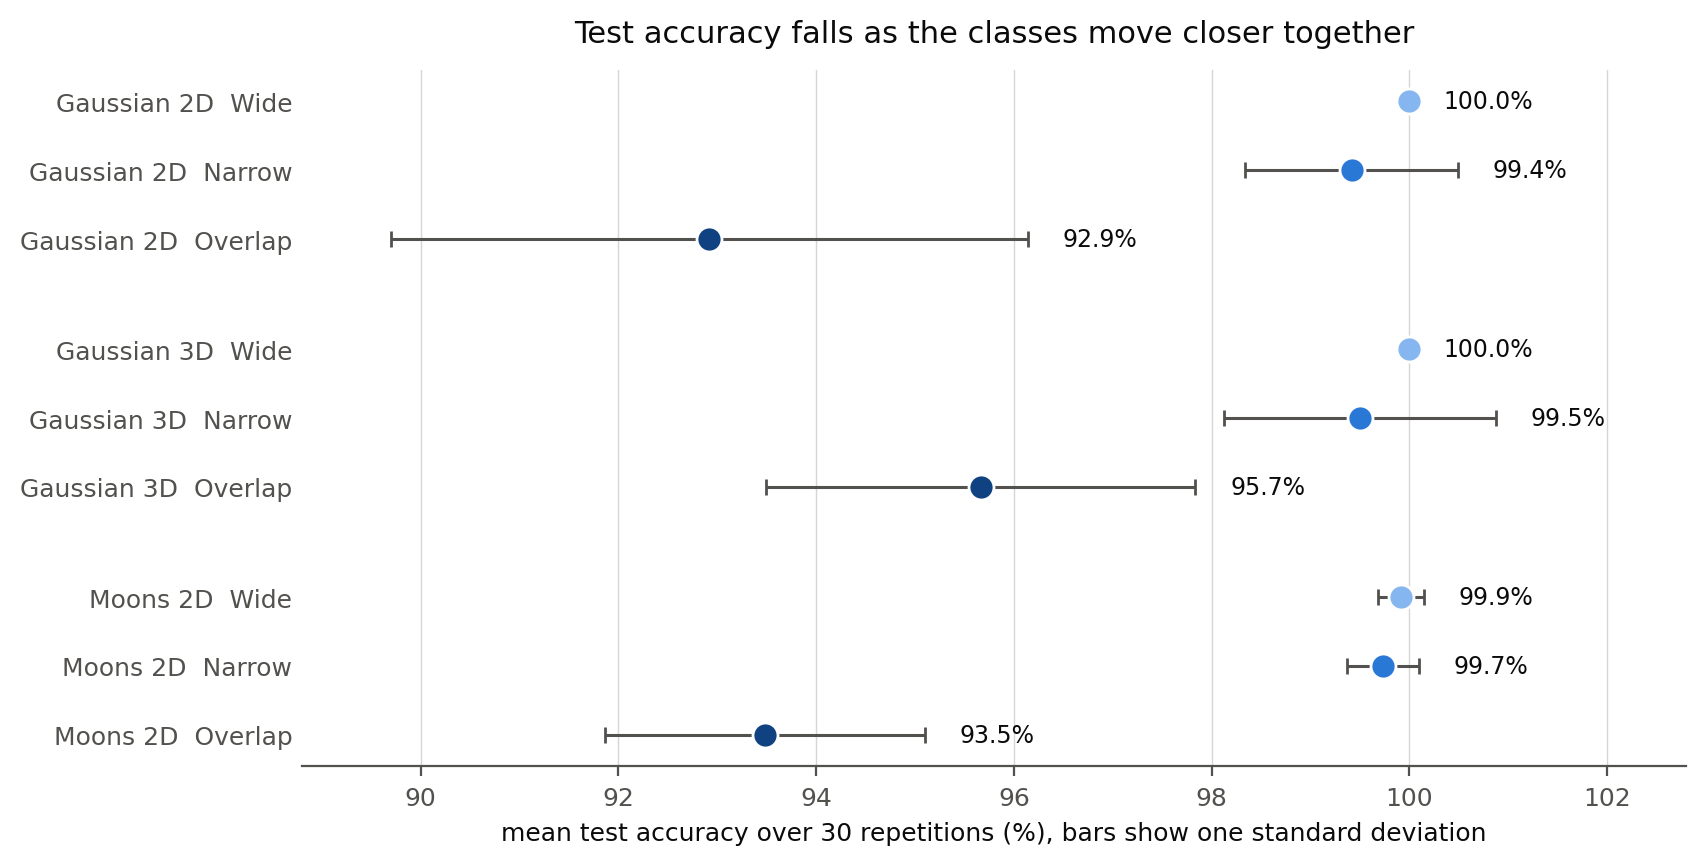
\includegraphics[width=0.95\textwidth]{../figures/fig5_accuracy.png}
\caption{Test accuracy across all nine datasets. A dot plot rather than bars,
because every value lies between 92 and 100 percent: bars drawn from zero would
be nine indistinguishable blocks, and bars drawn from 90 would exaggerate the
differences by cutting off the baseline that gives a bar its meaning.}
\label{fig:accuracy}
\end{figure}

\begin{figure}[H]
\centering
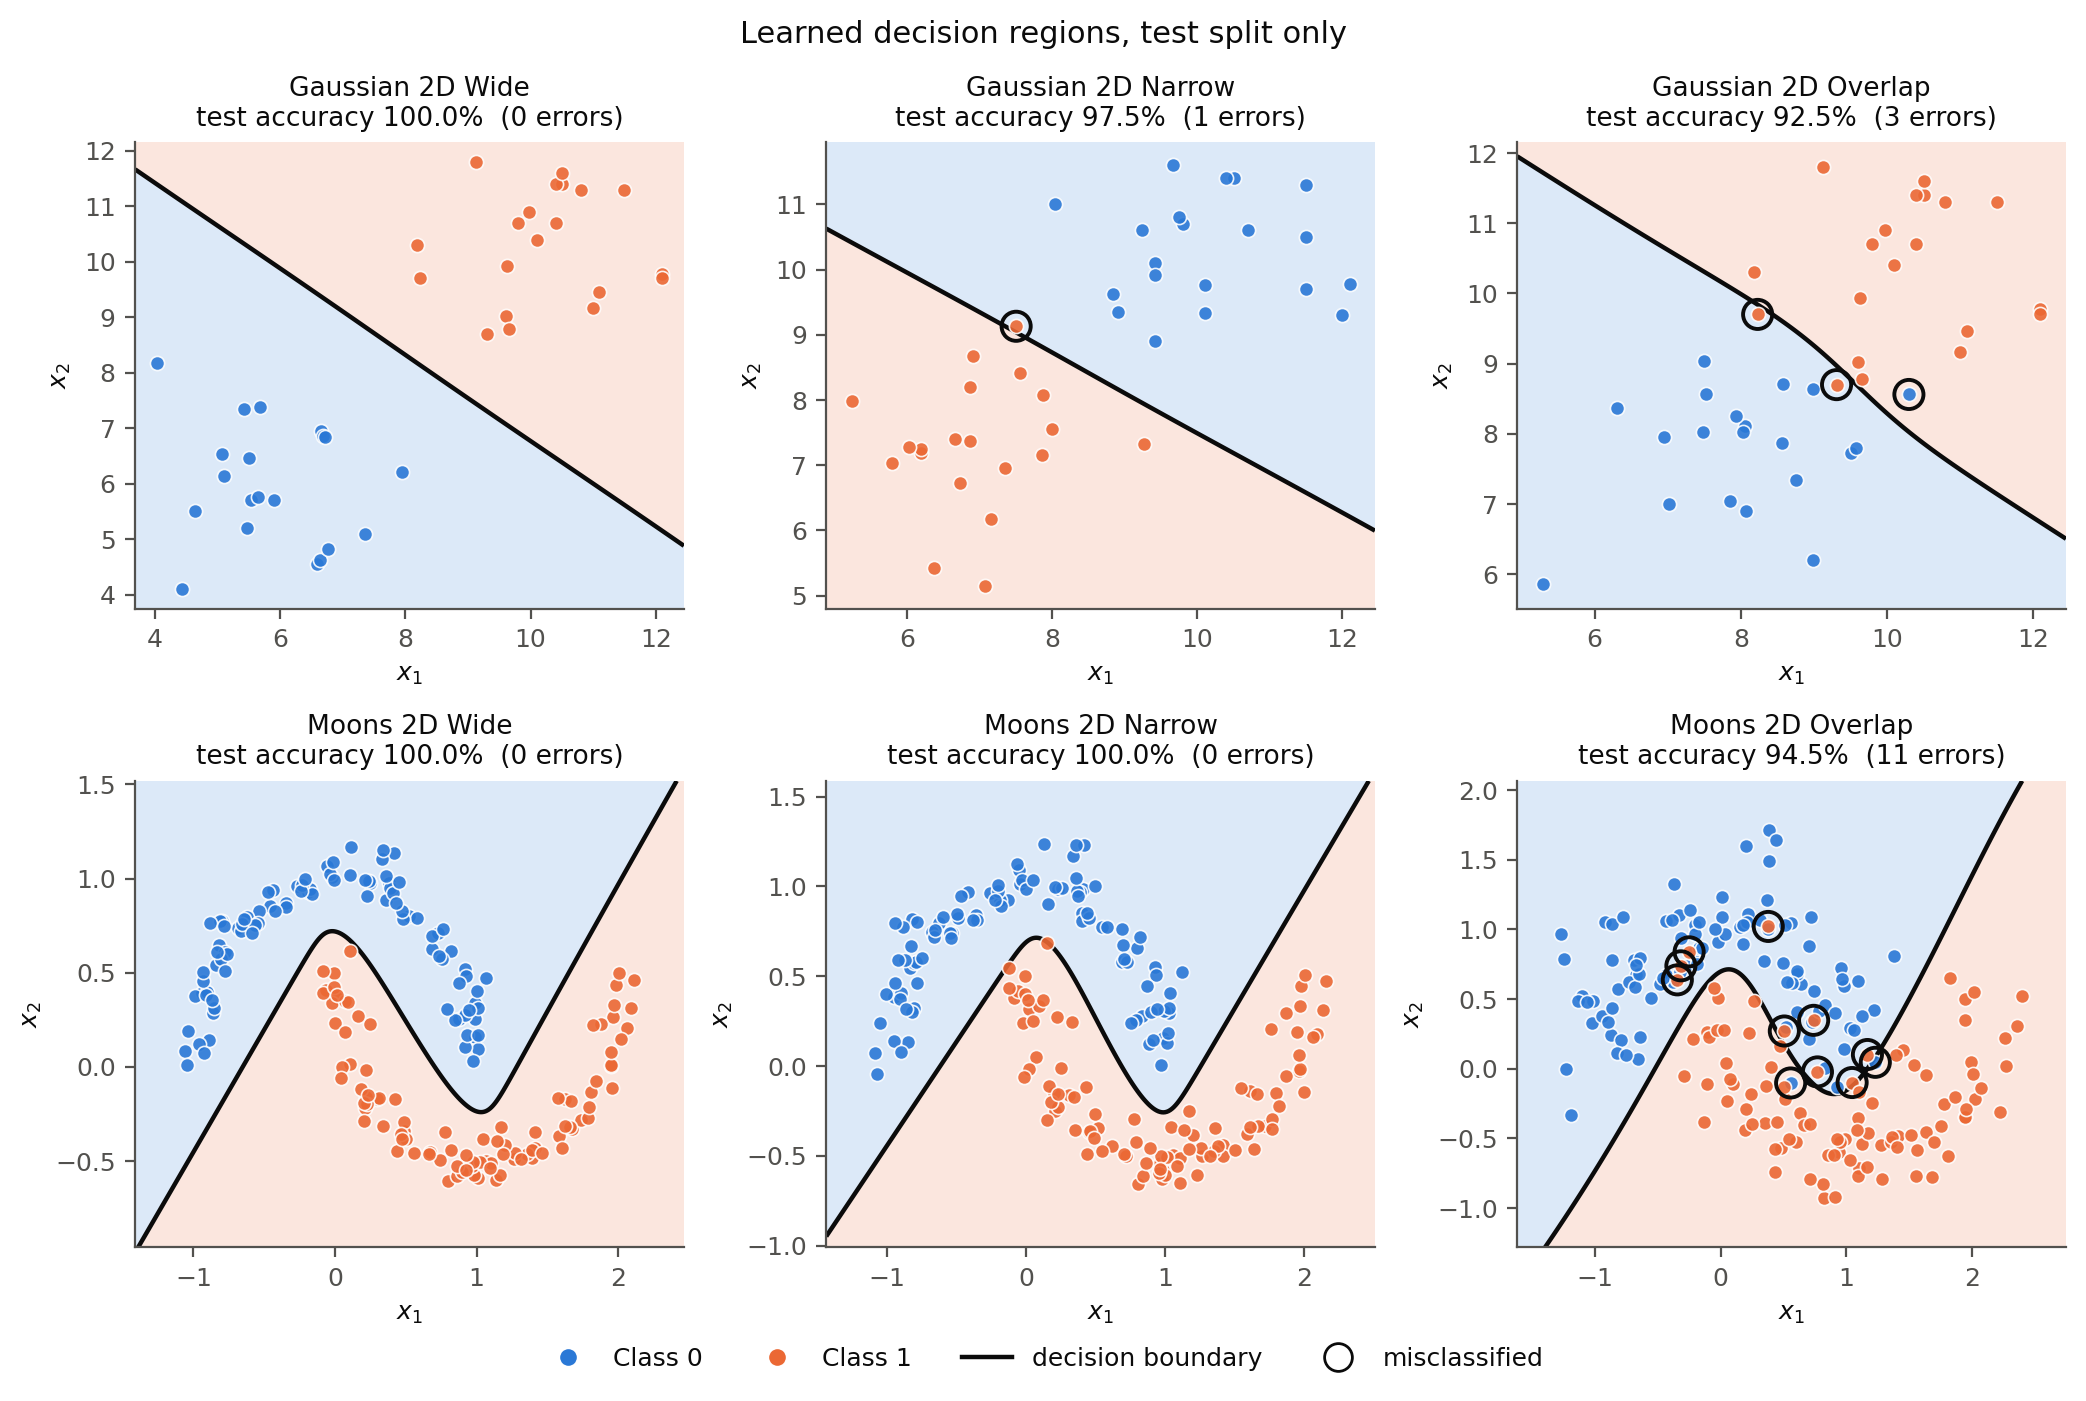
\includegraphics[width=\textwidth]{../figures/fig2_decision_regions.png}
\caption{Decision regions learned on the six two-dimensional datasets. Only
test points are shown; including the training points would make the boundary
look better than it is.}
\label{fig:regions}
\end{figure}

\begin{figure}[H]
\centering
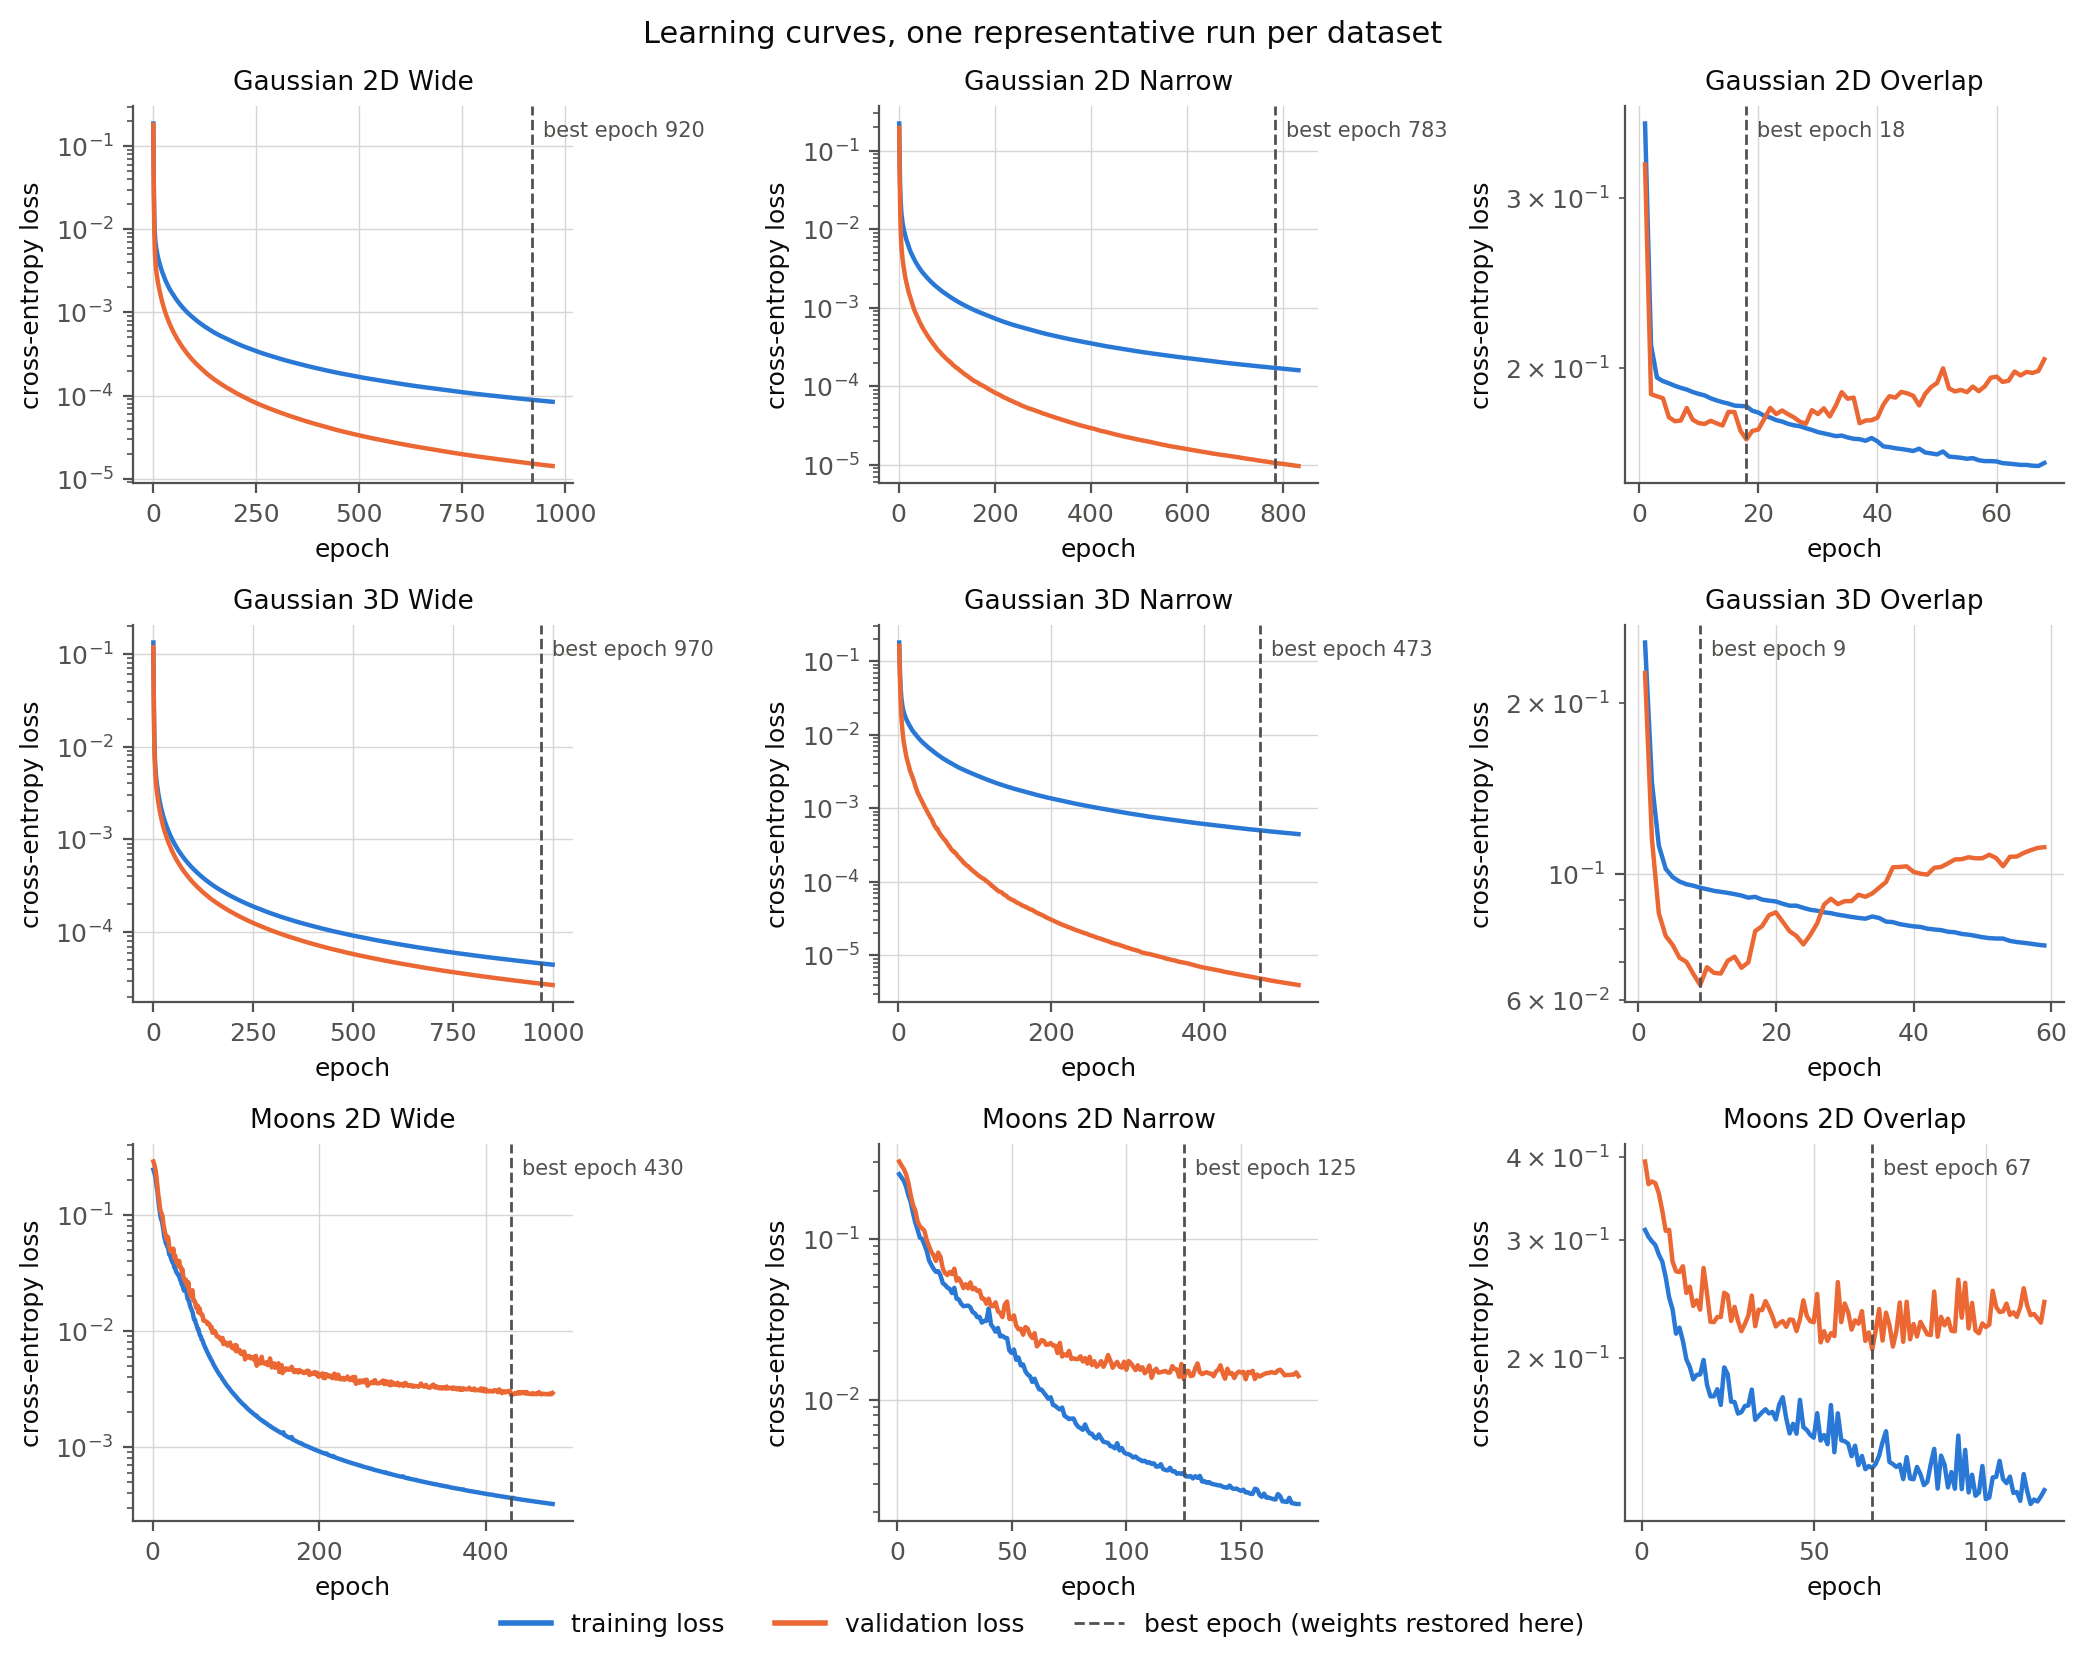
\includegraphics[width=\textwidth]{../figures/fig4_learning_curves.png}
\caption{Training and validation loss, log scale, for one representative run
per dataset. Note the contrast between the well-separated problems, where both
curves fall together indefinitely, and the overlapping problems, where
validation loss turns upward within twenty epochs.}
\label{fig:curves}
\end{figure}

\subsection{Gaussian 2D Wide (step 11)}

Mean test accuracy $100.00 \pm 0.00$ percent. Every one of the thirty runs
classified all forty test points correctly.

The two clusters are separated by more than five within-class standard
deviations, so a wide band of empty space sits between them and a great many
different boundaries would score perfectly. Figure~\ref{fig:regions} shows the
network placing an essentially straight line through the middle of that gap,
which is the sensible solution: with no data in the gap there is nothing to
curve around.

The interesting observation is the epoch count. This dataset ran to nearly the
full 1000-epoch cap, more than ten times longer than the overlapping variant,
despite being by far the easier problem. Early stopping never triggered because
the validation loss never stopped improving. On perfectly separable data the
cross-entropy loss can always be reduced further by scaling the weights up,
which pushes the sigmoid outputs closer to exactly 0 and 1 and increases the
margin. The network was therefore still making real progress on the loss long
after it had stopped making any progress on accuracy. This is worth flagging as
a limitation of loss-based early stopping on separable data.

\subsection{Gaussian 2D Narrow (step 13)}

Mean test accuracy $99.42 \pm 1.08$ percent, against an estimated ceiling of
98.9 percent. The network is at the ceiling.

Twenty-three of the thirty runs were perfect and the worst was 97.5 percent,
which on a 40-point test set means a single misclassified item. Precision (99.84)
slightly exceeds recall (99.00), so the few errors are marginally more often
Class 1 points assigned to Class 0 than the reverse, but with a mean of 0.20
false negatives per run against 0.03 false positives this is a difference of a
fraction of a point per run and I would not read anything into it.

\subsection{Gaussian 2D Overlap (step 15)}

Mean test accuracy $92.92 \pm 3.22$ percent, against an estimated ceiling of
92.5 percent. The network is at the ceiling.

This is the most informative of the Gaussian results, for two reasons.

First, the residual 7 percent error is not a failure of the network. The
estimated Bayes rate for these two fitted Gaussians is 92.5 percent, so an
optimal classifier with full knowledge of the generating distributions would
make roughly the same number of mistakes. The clusters genuinely interpenetrate,
and the misclassified points visible in Figure~\ref{fig:regions} sit in the
region where the other class is actually more probable. No amount of additional
capacity or training would fix them.

Second, this dataset has the largest run-to-run spread in the study, 3.22
percentage points, with individual runs ranging from 85.0 to 100.0 percent. Part
of that is the 40-point test set, where each error costs 2.5 points. But it also
reflects a real property of overlapping data: which points land in the test
split matters much more when many points sit near the boundary.

The learning curve for this dataset is the clearest illustration of overfitting
in the study. Validation loss bottoms out around epoch 18 and then climbs
steadily while training loss continues to fall, and training halts at epoch 89.
Without early stopping, the network would have kept contorting the boundary to
capture individual training points.

\subsection{Gaussian 3D Wide (step 17)}

Mean test accuracy $100.00 \pm 0.00$ percent, ceiling 100.0 percent.

The easiest problem in the set, with a separation index of 7.41. As with the 2D
Wide case, every run was perfect and training ran to the full 1000-epoch cap
without early stopping ever triggering, for the same reason. Figure~\ref{fig:3d}
shows the learned surface passing through the empty region between the two
clouds.

\subsection{Gaussian 3D Narrow (step 19)}

Mean test accuracy $99.50 \pm 1.38$ percent, ceiling 99.4 percent. At the
ceiling. Precision and recall are essentially identical at 99.52 and 99.50, so
the errors are symmetric between the classes.

\subsection{Gaussian 3D Overlap (step 21)}

Mean test accuracy $95.67 \pm 2.17$ percent, against a ceiling of 96.0 percent.
The network is within a third of a percentage point of the ceiling, which given
a 40-point test set is inside the resolution of the measurement.

Comparing this against Gaussian 2D Overlap gives the most useful single insight
in the study. The 3D version scores 95.67 percent while the 2D version scores
92.92, so the higher-dimensional problem is the \emph{easier} one. This runs
against the intuition that more dimensions make classification harder. The
explanation is in Table~\ref{tab:chars}: the 3D Overlap classes have a
separation index of 3.66 against 2.96 for the 2D version. The third coordinate
carries genuine discriminative information, and adding an informative dimension
pushes the classes further apart in the space where the separation actually
happens. Dimensionality hurts when the added dimensions are noise; it helps when
they are signal.

\begin{figure}[H]
\centering
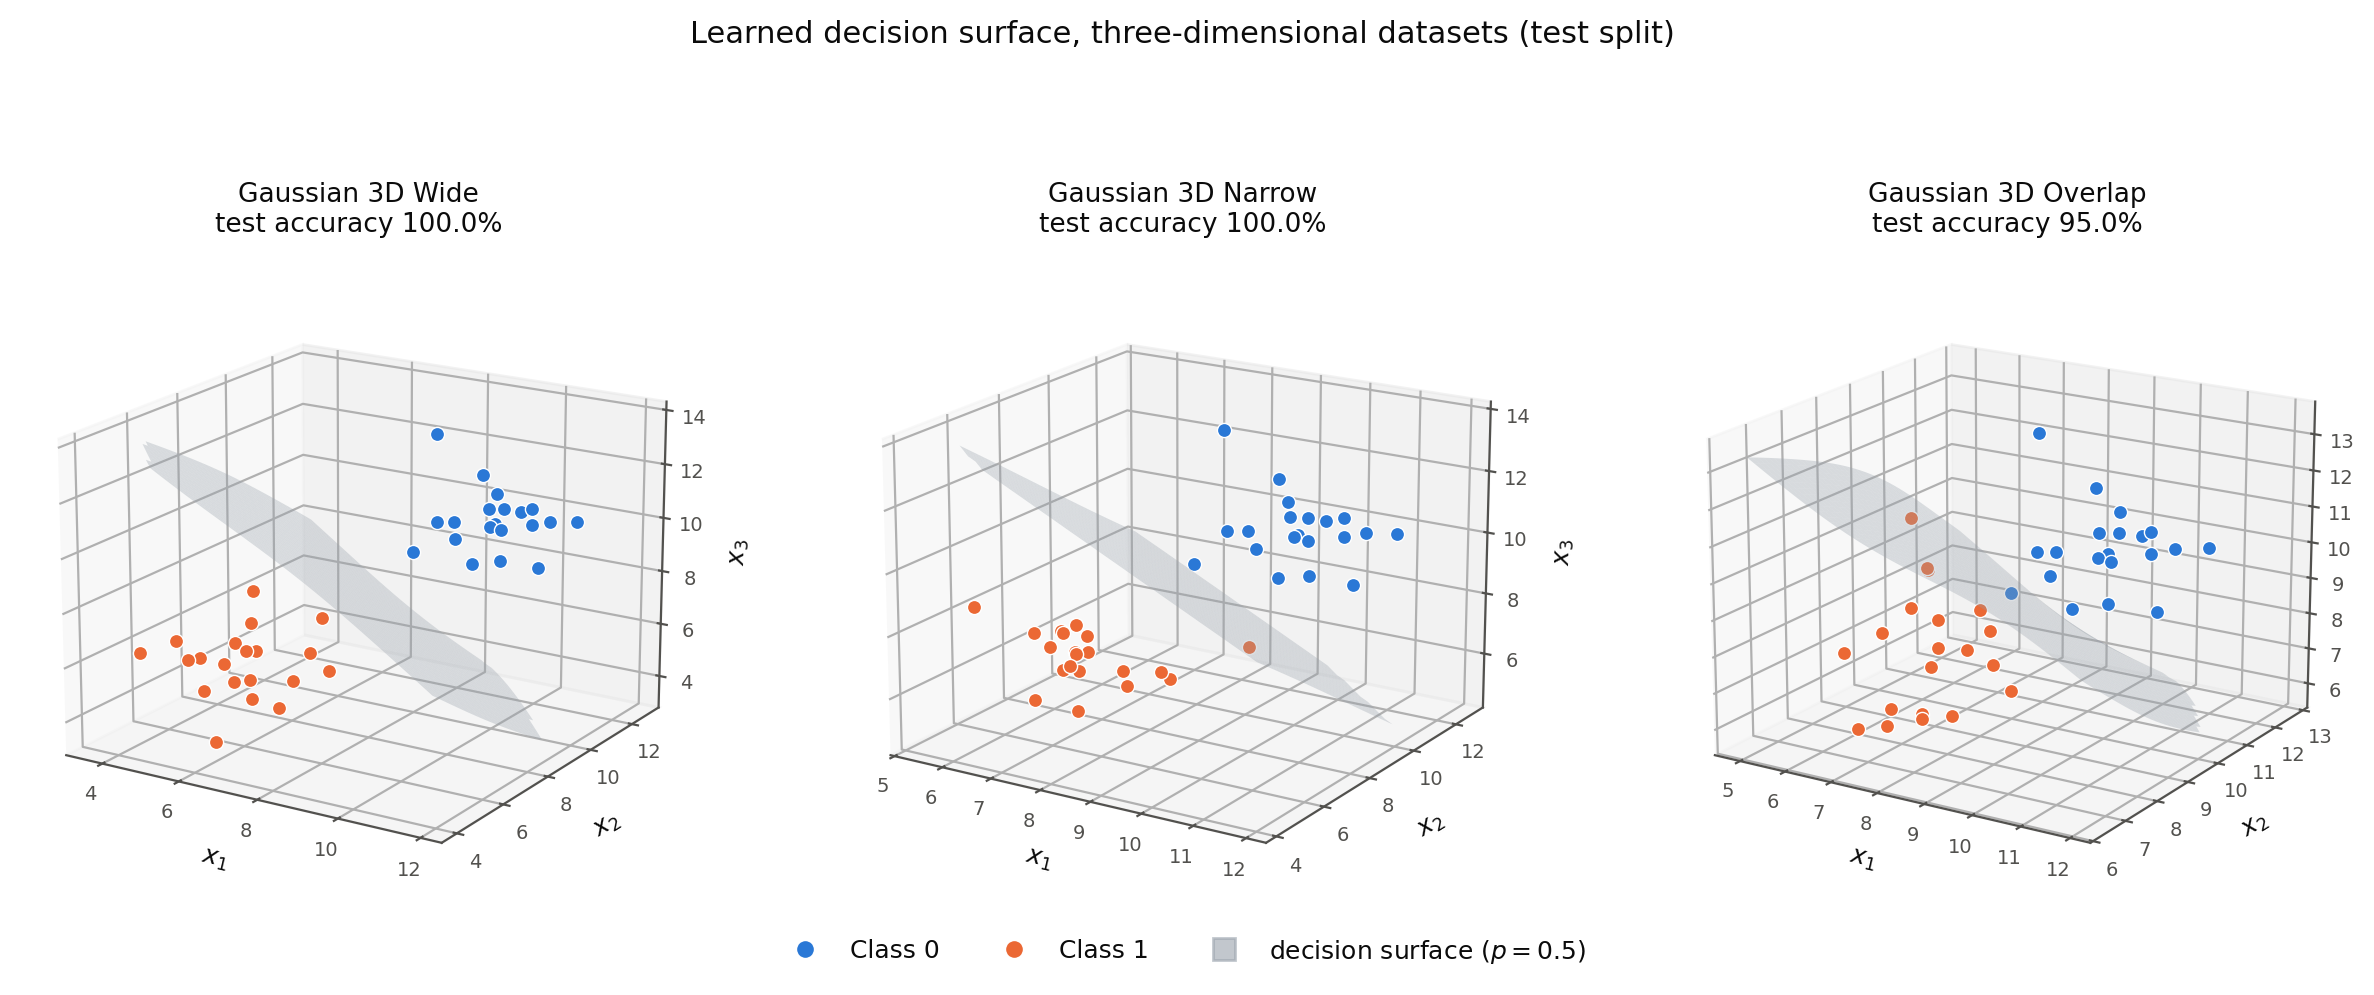
\includegraphics[width=\textwidth]{../figures/fig3_decision_3d.png}
\caption{Learned decision surface for the three-dimensional datasets, shown on
the test split. The surface is the set of points where the network outputs 0.5,
traced by scanning along $x_3$ and interpolating the crossing.}
\label{fig:3d}
\end{figure}

\subsection{Moons 2D Wide (step 23)}

Mean test accuracy $99.92 \pm 0.23$ percent, ceiling 99.9 percent. At the
ceiling.

This dataset is the real test of whether the hidden layer is doing its job. The
two moons interlock, so no straight line can separate them: any line that cuts
off the upper crescent must also cut through the lower one. Figure
\ref{fig:regions} shows the network producing a curved boundary that follows the
channel between the two arcs, which is only possible because the hidden units
are combining into a non-linear function. A single artificial neuron of the kind
studied in Homework 1 would be incapable of this, and would be limited to
roughly the accuracy of the best available straight line.

With 200 test points instead of 40, the accuracy resolution here is 0.5
percentage points rather than 2.5, so these numbers are considerably more
precise than the Gaussian ones.

\subsection{Moons 2D Narrow (step 25)}

Mean test accuracy $99.73 \pm 0.37$ percent, ceiling 99.7 percent. At the
ceiling, and barely distinguishable from the Wide variant.

This is worth noting: for the moons, narrowing the gap between Wide and Narrow
costs almost nothing, only 0.19 percentage points, whereas for the Gaussians the
same step costs 0.58. The reason is visible in Table~\ref{tab:chars}. The moons
Wide and Narrow variants have nearly identical separation indices (2.46 against
2.44), so despite the labels they are close to the same problem in difficulty.
The label describes how the data was generated rather than how hard it is to
classify.

\subsection{Moons 2D Overlap (step 27)}

Mean test accuracy $93.48 \pm 1.62$ percent, against an estimated ceiling of
94.6 percent.

This is the one dataset where the network leaves measurable headroom, about 1.1
percentage points.

My first explanation was that eight tanh units are too few to trace the boundary
between two interpenetrating crescents, and that more capacity would close the
gap. Section~\ref{sec:capacity} reports the experiment I ran to check that, and
the answer is that the explanation is wrong. Widening the hidden layer from four
units to sixty-four changes nothing, and two hidden layers change nothing
either. The residual error is not a shortage of model capacity.

The errors are symmetric (precision 93.36, recall 93.70, with 6.73 false
positives against 6.30 false negatives per run). Figure~\ref{fig:regions} shows
them concentrated exactly where the two crescents interpenetrate, which is the
expected pattern.

\subsection{Does more capacity close the Moons Overlap gap?}
\label{sec:capacity}

Moons 2D Overlap is the only dataset that finished below its estimated ceiling,
so it is the only place where the question "could a different network have done
better?" has a chance of a yes. My stated suspicion was that eight tanh units
are too few for the boundary between two interpenetrating crescents. That is a
testable claim, so I tested it rather than leaving it as an assertion.

The hidden layer was swept from four units to sixty-four, plus a two-layer
configuration, with thirty repetitions at every setting. Gaussian 2D Overlap was
run as a control: it is already at its ceiling and its optimal boundary is close
to a straight line, so if capacity were the mechanism it should help the moons
and not the Gaussian.

\begin{table}[H]
\centering
\small
\begin{tabular}{lrrrr}
\toprule
Hidden layer & Parameters & Test accuracy & Training accuracy & Epochs \\
\midrule
\multicolumn{5}{l}{\emph{Moons 2D Overlap, estimated ceiling 94.6\%}} \\
(4)      &  17 & $94.12 \pm 1.30$ & 94.50 & 158 \\
(8)      &  33 & $93.48 \pm 1.62$ & 94.17 & 170 \\
(16)     &  65 & $93.73 \pm 1.51$ & 94.40 & 192 \\
(32)     & 129 & $93.70 \pm 1.40$ & 94.20 & 174 \\
(64)     & 257 & $93.72 \pm 1.62$ & 94.11 & 170 \\
(16, 16) & 337 & $93.68 \pm 1.46$ & 94.17 & 114 \\
\addlinespace
\multicolumn{5}{l}{\emph{Gaussian 2D Overlap, estimated ceiling 92.5\%}} \\
(4)      &  17 & $92.92 \pm 3.54$ & 93.56 & 108 \\
(8)      &  33 & $92.92 \pm 3.22$ & 93.17 &  89 \\
(16)     &  65 & $92.58 \pm 3.97$ & 93.28 &  90 \\
(32)     & 129 & $92.75 \pm 3.37$ & 92.97 &  80 \\
(64)     & 257 & $93.00 \pm 3.68$ & 93.03 &  69 \\
(16, 16) & 337 & $92.92 \pm 3.72$ & 93.33 &  90 \\
\bottomrule
\end{tabular}
\caption{Capacity sweep, 30 repetitions per setting. Nothing moves. The
parameter count varies by a factor of twenty and test accuracy varies by less
than the run-to-run standard deviation.}
\label{tab:capacity}
\end{table}

\begin{figure}[H]
\centering
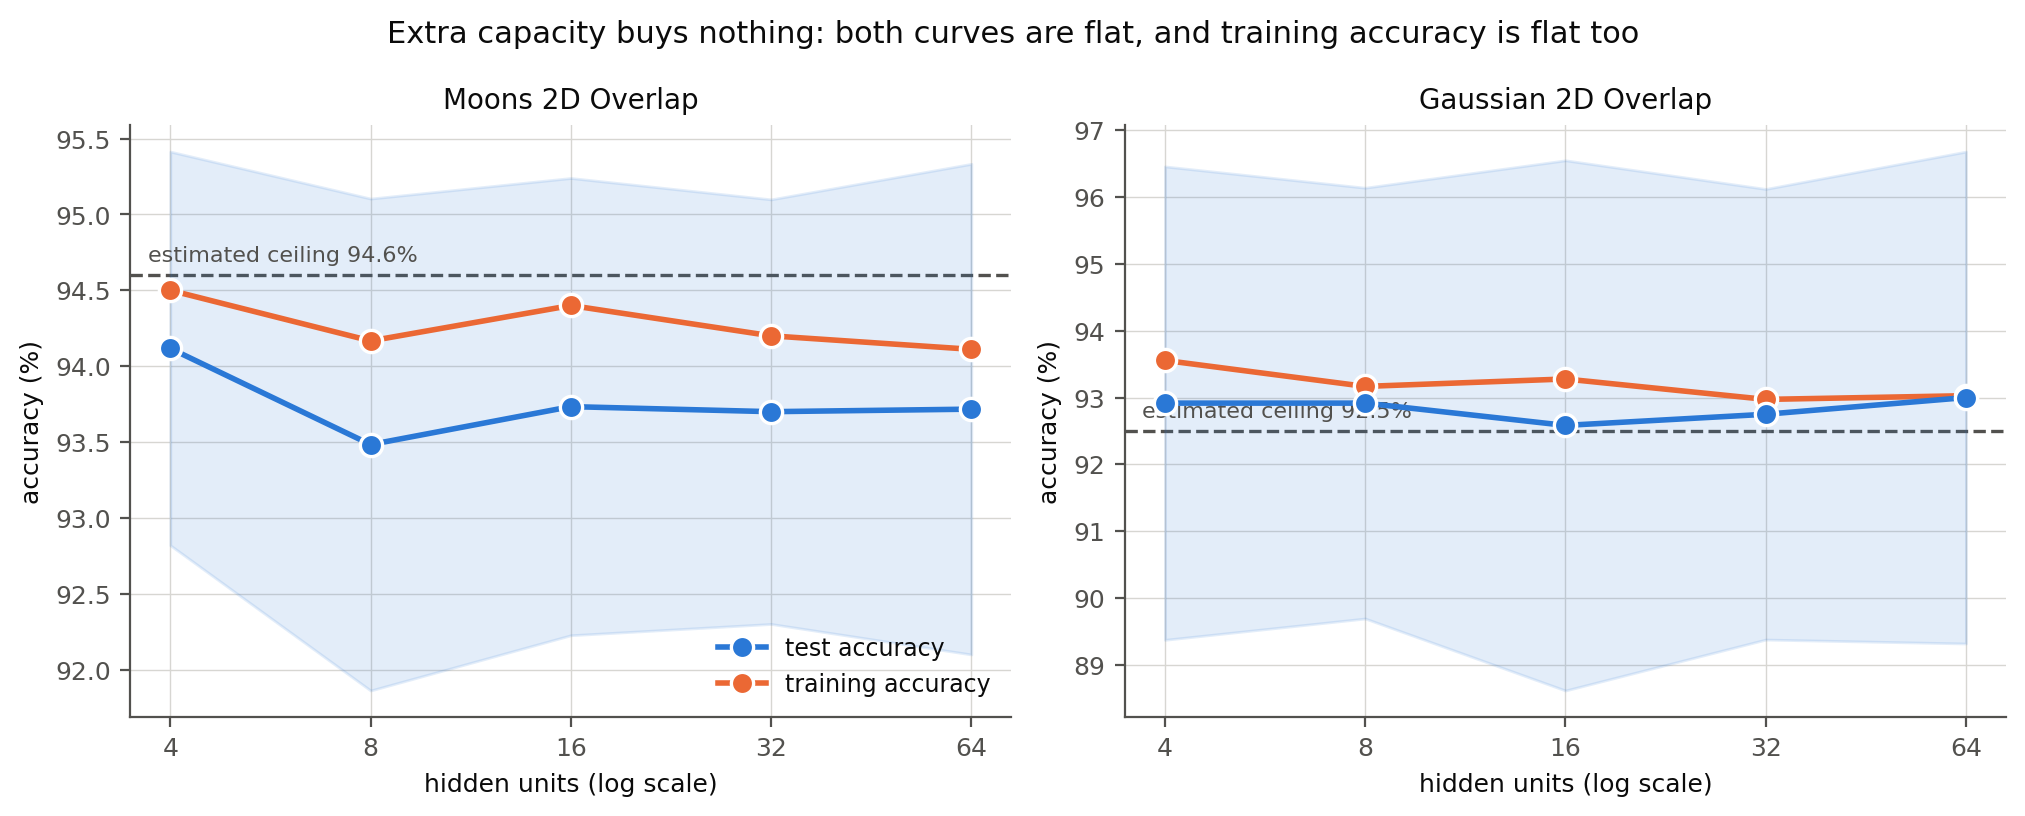
\includegraphics[width=0.95\textwidth]{../figures/fig6_capacity.png}
\caption{Accuracy against hidden-layer width on the two overlapping datasets.
The shaded band is one standard deviation on test accuracy. Both curves are
flat, and so is the training curve, which is the part that settles the
question.}
\label{fig:capacity}
\end{figure}

\paragraph{The claim was wrong.} Extra capacity does not help. On the moons, a
paired comparison across the same thirty seeds puts four units 0.63 points
\emph{above} eight ($p = 0.014$), and sixty-four units indistinguishable from
eight ($p = 0.42$). If anything the narrowest network is the best of them, which
is the opposite of a capacity shortage.

\paragraph{The training accuracy is what proves it.} The decisive column in
Table~\ref{tab:capacity} is not the test column but the training one. Training
accuracy sits between 94.1 and 94.5 percent at every width. A network with
sixty-four hidden units and 257 parameters cannot fit 600 training points any
better than one with four units and 17 parameters. If the problem were
insufficient capacity, the larger network would at minimum fit the training data
better, even at the cost of generalizing worse. It does not. The network has
already extracted all the structure the data contains, and the remaining errors
are points that genuinely sit on the wrong side of the true boundary.

\paragraph{So what explains the 1.1 point gap?} Most likely the ceiling estimate
rather than the network. The moons ceiling comes from leave-one-out
15-nearest-neighbour accuracy, which is a biased estimator on a finite sample:
it can flatter itself on 1000 points by effectively memorizing local
neighbourhoods. Reading the evidence together, the honest conclusion is that
Moons 2D Overlap is at its ceiling too, and that the apparent shortfall is an
artifact of how the ceiling was estimated. This would have been invisible
without running the sweep.

\paragraph{What I would revise.} Design choice 3 selected eight hidden units on
validation accuracy. On this evidence four would have been the better choice for
the overlapping problems, giving the same accuracy with half the parameters. I
have left the reported results at eight units, because changing the architecture
after seeing test results is exactly the kind of decision that invalidates a
held-out test set, and reporting the number I committed to is more honest than
reporting the best number I found.

\subsection{Overall conclusions}

\paragraph{The network works, and it works up to the limit of the data.}
On eight of the nine datasets the measured accuracy is at or above the estimated
Bayes ceiling. The ninth, Moons 2D Overlap, appeared to fall 1.1 points short,
but the capacity experiment in Section~\ref{sec:capacity} indicates that the
shortfall lies in the ceiling estimate rather than in the network: no amount of
extra capacity improves it, and crucially none improves the \emph{training}
accuracy either.
On a few datasets the measured accuracy sits marginally above the estimated
ceiling, which is a sampling artifact rather than a real result: the ceiling is
estimated from densities fitted to the whole dataset while accuracy is measured
on 40 or 200 held-out points, and those two quantities have independent errors.

\paragraph{Accuracy tracks class separation, not dimensionality and not
sample size.} Within every family, accuracy falls monotonically from Wide to
Narrow to Overlap. Across families, the ordering is predicted by the separation
index in Table~\ref{tab:chars} rather than by the number of dimensions or the
number of samples. The clearest evidence is Gaussian 3D Overlap outscoring
Gaussian 2D Overlap.

\paragraph{The hidden layer is doing real work, but only where it is needed.}
On the Gaussian problems the learned boundary is nearly straight, because the
optimal boundary for two roughly spherical Gaussians is close to a hyperplane.
On the moons it is strongly curved. The same architecture produced both, which
is the point of a hidden layer: the capacity is available when the problem needs
it and is not forced onto problems that do not.

\paragraph{Early stopping matters on hard problems and is inert on easy ones.}
The overlapping datasets stop within 80 to 170 epochs with validation loss
already rising. The well-separated datasets run to the 1000-epoch cap without
ever triggering it. This asymmetry is not a bug; it reflects the fact that
overfitting is only possible when there is noise to fit.

\paragraph{A speculation worth testing turned out to be wrong.} I wrote in an
earlier draft that eight hidden units were probably too few for the moons
boundary. The capacity sweep refuted that cleanly, and the diagnostic that
settled it was training accuracy rather than test accuracy. That is the most
useful methodological lesson in this project for me: when a model underperforms,
the first question is not "is the model too small?" but "can a bigger model even
fit the training data better?". If it cannot, capacity is not the constraint and
no amount of architecture search will help.

\paragraph{The main methodological weakness is test set size.} Forty test
points on the Gaussian problems means accuracy is quantized to 2.5 percentage
point steps. Thirty repetitions substantially mitigate this for the mean, but
the reported standard deviations for the Gaussian datasets are inflated by
quantization and should not be compared directly against the moons figures. If I
could change one thing about the experimental design, it would be to use
repeated $k$-fold cross-validation instead of a single holdout split, which
would use every point for testing exactly once per repetition.

\section{Code and data organization}

\begin{table}[H]
\centering
\small
\begin{tabular}{p{4.6cm}p{9.9cm}}
\toprule
\textbf{Path} & \textbf{Contents} \\
\midrule
\texttt{src/ann.py} &
The network itself: forward pass, backpropagation, mini-batch SGD with
momentum, early stopping, and the gradient checker. \\
\texttt{src/data.py} &
Reading the CSVs, the stratified split, the standardizer, and the metric
calculations. \\
\texttt{src/experiment.py} &
The architecture grid search and the repeated evaluation runs. Running it
reproduces every number in this report. \\
\texttt{src/analysis.py} &
Dataset characterisation and the Bayes ceiling estimates. \\
\texttt{src/capacity.py} &
The hidden-layer capacity sweep behind Section~\ref{sec:capacity}. \\
\texttt{src/plots.py} &
All five figures. \\
\texttt{data/} &
The nine CSV files exactly as provided, renamed only to remove spaces. \\
\texttt{results/all\_runs.csv} &
One row per run, 270 rows. Every metric recorded for every repetition. \\
\texttt{results/summary.csv} &
One row per dataset: mean, standard deviation, minimum and maximum. \\
\texttt{results/architecture\_search.csv} &
The grid search results behind Section~\ref{sec:arch}. \\
\texttt{results/dataset\_characteristics.csv} &
Separation indices and ceiling estimates behind Table~\ref{tab:chars}. \\
\texttt{results/capacity\_sweep.csv} &
The capacity sweep results behind Table~\ref{tab:capacity}. \\
\texttt{figures/} &
The five figures as PNG. \\
\bottomrule
\end{tabular}
\end{table}

To reproduce everything from a clean checkout:
\begin{verbatim}
    pip install numpy matplotlib
    cd src
    python3 experiment.py     # grid search + 270 runs, about 4 minutes
    python3 analysis.py       # dataset characteristics and ceilings
    python3 capacity.py       # capacity sweep, about 1 minute
    python3 plots.py          # all figures
\end{verbatim}

\texttt{results/all\_runs.csv} holds the raw per-run data. Each row records the
dataset, the seed, the split sizes, the number of epochs run, the best epoch,
training time, the loss on each split, and accuracy, precision, recall, F1 and
the four confusion counts for each of the training, validation and test splits.

\section{Credit and sources}

\paragraph{Code.} All source code is original and was written for this
assignment. It was not derived from an existing implementation, and no machine
learning library was used: NumPy provides array arithmetic and matplotlib
provides plotting, and nothing else is imported. The backpropagation
derivation followed is the standard one presented in Mitchell chapter 4 and in
the course lecture slides on artificial neural networks; the algorithm is
textbook material, the implementation of it is mine.

\paragraph{Ideas and methods.} The Xavier/Glorot initialization scheme is due to
Glorot and Bengio (2010). The sigmoid-with-cross-entropy gradient
simplification in design choice 6 is standard and is derived in most
treatments of the topic. The use of a Bayes-rate estimate as a reference
ceiling is a standard evaluation practice rather than my invention.

\paragraph{AI assistance.} I used an AI assistant (Claude) while working on this
assignment, as permitted by the course. It was used for implementation, for
running the experiments, and for drafting this document. I reviewed the design
choices, the results and the conclusions, and I am responsible for the content
of what is submitted.

\paragraph{Data.} All nine datasets were supplied with the assignment. The files
were renamed only to remove spaces from the filenames; their contents are
unmodified.

\end{document}
